\subsection{业务代表模式}

业务代表模式是一种软件设计模式,它的目的是通过抽象化和封装来减少系统中对象之间的依赖。业务代表模式通过引入一个中介对象(称为业务代表)来处理复杂的业务逻辑,从而减少对象之间的直接依赖关系。

业务代表模式通常用于分离复杂的业务逻辑,使系统中的对象可以更简单地进行单元测试。例如,如果您有一个复杂的业务对象,它与数据库进行交互,并且需要进行大量的计算来完成其工作,那么您可以使用业务代表模式来抽象出这些复杂的操作,从而使您的业务对象变得更简单,更容易测试。

业务代表模式还可以用于分离系统中不同模块之间的依赖关系。例如,如果您有一个业务对象,它依赖于另一个模块来执行某些操作,那么您可以使用业务代表模式来分离这些操作,使得您的业务对象不再依赖于其他模块。这样一来,您就可以更容易地对每个模块进行单独的测试和维护。

业务代表模式的优点如下:
\begin{enumerate}
\item 业务代表模式可以将复杂的业务逻辑封装起来,从而使得业务逻辑更加清晰、易于维护。
\item 业务代表模式可以有效地隔离应用程序的用户界面和业务逻辑,从而使得应用程序更加松耦合,更容易实现模块化。
\item 业务代表模式提供了一种统一的访问入口,使得用户可以更方便地访问业务逻辑。
\item 业务代表模式可以实现业务逻辑的灵活扩展,从而使得应用程序能够适应不断变化的需求。
\end{enumerate}

业务代表模式的缺点如下:
\begin{enumerate}
\item 业务代表模式可能导致系统变得过于复杂,从而增加系统维护的难度。
\item 业务代表模式的实现可能会增加系统的开发和维护成本。
\item 业务代表模式可能会导致系统的性能下降,因为需要进行大量的数据传递和处理。
\item 业务代表模式的实现可能会带来安全隐患,因为业务逻辑的封装可能会导致安全漏洞难以发现和修复。
\end{enumerate}



\begin{figure}[htb]
  \centering
  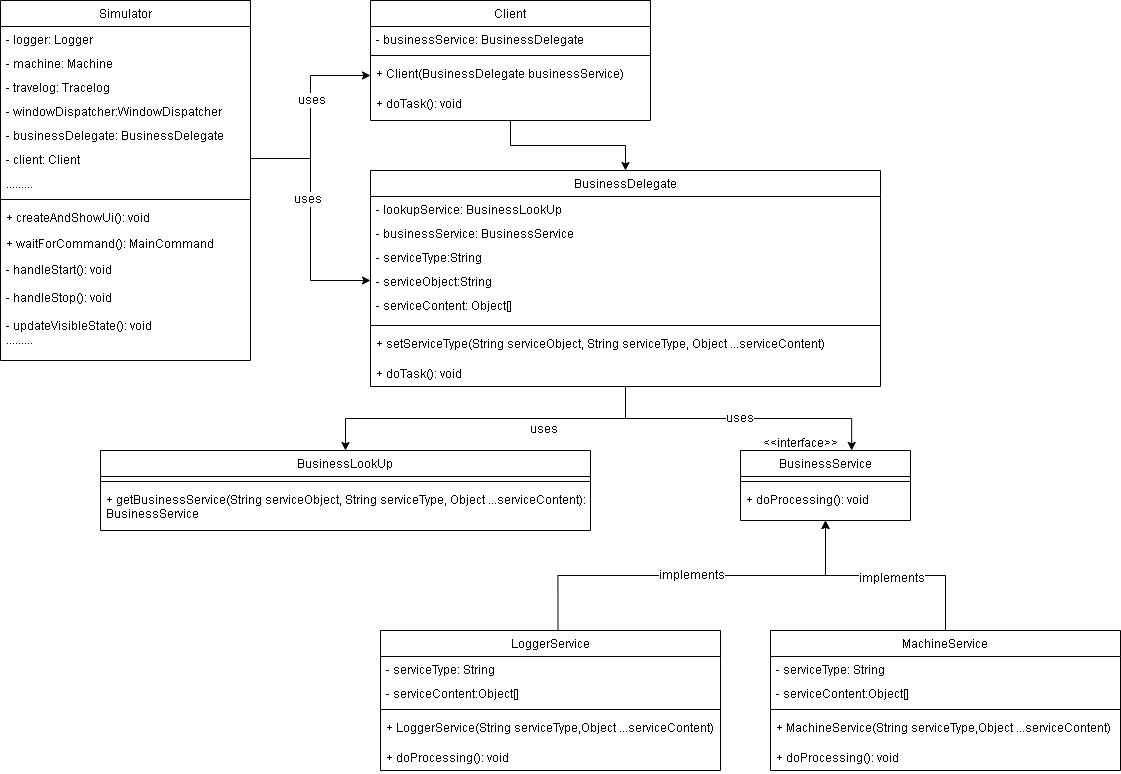
\includegraphics[width=0.9\textwidth]{figures/业务代表模式.png}
  \caption{业务代表模式在 Slow6502 中的类图}
\end{figure}
